\documentclass[11pt,openany,twoside]{report}
\usepackage[utf8]{inputenc}
\usepackage[hmargin=4cm,vmargin=3.5cm,bmargin=3.5cm]{geometry}
\usepackage[portuguese, english]{babel}
\usepackage{graphicx}
\usepackage{hyperref}
\usepackage{indentfirst}

\title{\textbf{Relatório - Bases de Dados}}

\begin{document}

\begin{titlepage}
\begin{figure}
\title{\textbf{Relatório - Bases de Dados}}
\author{Turma 2 - Diogo Daniel Soares Ferreira e Luís Davide Leira\\\vspace{3cm}
Universidade de Aveiro - Laboratórios de Informática}
\date{\today}
 
\includegraphics[scale=1.5]{ua_logo.png}
\end{figure}
\end{titlepage}

\selectlanguage{portuguese}
\maketitle
\tableofcontents
\listoffigures

\part{Apresentação}

\chapter{Resumo}

Uma base de dados é uma coleção de dados correlacionados entre si com diversos fins. Estes sistemas são de importância tal que nos deparamos e lidamos com eles no nosso quotidiano. É inegável o facto de conferirem organização, consistência e uma forma intuitiva de armazenamento de dados. 

Ao longo do relatório é abordada a base de dados criada e sua composição, o planeamento e o funcionamento de uma aplicação desenvolvida que permite a gestão da base de dados, sendo ela uma biblioteca onde se pretende armazenar informação sobre utilizadores, livros e suas requisições. A aplicação apresenta uma interface composta por menus que permitem a realização de operações simples que asseguram o funcionamento da biblioteca em questão.

Sucintamente, a aplicação é capaz de localizar livros (por autor, título ou estado), listar utilizadores e requisições de utilizadores, criar, alterar ou apagar elementos tais como
utilizadores, livros e requisições. Esta foi desenvolvida sempre com um método de programação defensivo, assegurando maior estabilidade e flexibilidade. No entanto, revela ser demasiado básica para ser utilizada em contextos mais exigentes a nível profissional, sendo apenas um exemplo de base de dados e de aplicação que assegura o funcionamento correto da mesma. Transmite de uma forma simplista os conceitos base para se poder trabalhar com este tipo de sistemas.

\chapter{Introdução}

Bases de dados são sistemas essenciais para o armazenamento de informação. Tratam-se de conjuntos de dados relacionados entre si de maneira simples e eficaz, capaz de organizar, armazenar ou apagar informação em poucas operações. Há vários modelos de bases de dados, sendo os modelos plano, hierárquico e o relacional os mais usados. Neste relatório, serão tratadas apenas as bases de dados relacionais.

\begin{figure}
 \center
 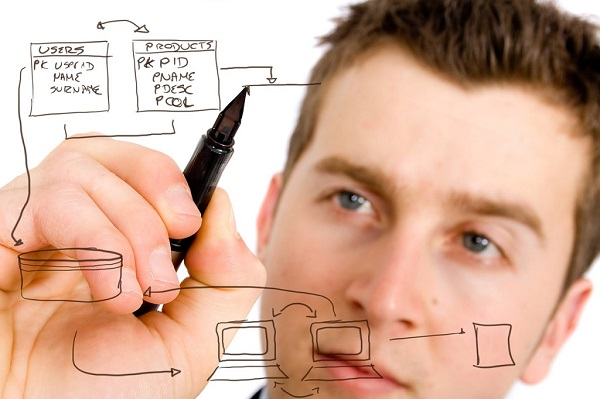
\includegraphics[scale=1.5]{database_plan.jpg}
 \caption{Exemplo do planeamento de uma base de dados relacional. Fonte: Flickr, tec\_estromberg}
 \label{database_plan}
\end{figure}

Surgidas em meados dos anos setenta, as bases de dados relacionais tratam a informação em tabelas (matematicamente falando, relações), podendo estar relacionadas entre si (\autoref{database_plan}). A linguagem padrão deste tipo de bases de dados é \textit{SQL}, que será usada ao longo deste relatório. Edgar Codd, em 1985, criou o modelo relacional, com treze regras fundamentais para a construção de uma base de dados sólida e com o mínimo de dependências entre tabelas. Não se irá aprofundar o modelo relacional ao longo do relatório, sendo a explicação mais detalhada encontrada no link \url{http://pt.wikipedia.org/wiki/Modelo\_relacional}.

O objetivo deste relatório é a exposição de uma aplicação codificada em Python 2.x capaz de lidar com uma base de dados simples semelhante à de uma biblioteca. A base de dados contém livros e utilizadores, que poderão requisitar livros. Através de um menu intuitivo ao utilizador, a aplicação terá de localizar, listar criar, alterar e apagar diversos elementos que compõem a base de dados.

Será utilizado o módulo SQLite3 presente na biblioteca de Python, o qual foi abordado e trabalho nas aulas de Laboratórios de Informática. Através de uma aplicação simples, é possível desempenhar tarefas que permitem o armazenamento e a manipulação de dados.

\part{Desenvolvimento}

\chapter{A base de dados}

Antes de ser desenvolvida qualquer aplicação, é necessário haver uma base de dados para armazenar dados e posteriormente ser manipulada pela aplicação que era pretendido fazer inicialmente. Foi necessário formular as tabelas que inserimos na base de dados, as quais permitem organizar a informação introduzida. Neste caso específico, optou-se por desenhar três tabelas:
\begin{itemize}
\item Criou-se uma tabela para os utilizadores chamada de \textit{users} com dois campos: \textit{Id\_User}, um inteiro que se irá incrementar automaticamente, a partir do número 1, e que serve de chave primária para cada utilizador; \textit{User\_Name}, um texto que irá identificar o utilizador, sendo que não poderão existir dois utilizadores com o mesmo \textit{User\_Name}.
\item Criou-se outra tabela para os livros chamada de \textit{books} com quatro campos: \textit{Id\_Book}, um inteiro que se irá incrementar automaticamente, a partir do número 1, servindo de chave primária para cada livro; \textit{Book\_Name}, um texto que será o título do livro; \textit{Author}, um texto que identificará o autor do livro; \textit{Book\_State}, que contém o estado atual de requisição do livro (podendo assumir o estado disponível ou requisitado).
\item Por fim, criou-se uma tabela específica para as requisições chamada \textit{requisitions}. Apesar de poder ser integrado na tabela dos livros, foi tirada a conclusão que seria mais fácil e lógico organizar a informação da requisição noutra tabela. Logo, essa tabela terá quatro campos: \textit{Id\_Book}, que representará o livro requisitado; \textit{Id\_User}, que representará o utilizador que requisitou o livro; \textit{Start\_date}, que representará a data em que o livro foi requisitado; \textit{End\_date}, que será uma data introduzida pelo utilizador para limite de entrega do livro.
\end{itemize}

\chapter{A aplicação}

\subsection{Planeamento da aplicação}

A aplicação começou por ser desenvolvida para correr apenas com os parâmetros de chamada, através da linha de comandos. Após algum trabalho já desenvolvido, concluiu-se que dessa maneira seria impossível descodificar a entrada para a codificação \textit{utf-8}, pois apenas é possível descodificar as entradas caso sejam feitas em tempo de execução, e não antes do programa executar. Isto causaria erros aquando da conversão do texto recebido para base de dados (caso fosse acentuado, por exemplo). Portanto, após um período de discussão, decidiu-se fazer um menu com uma interface hierárquica, que fosse simples e intuitivo para o utilizador. Também foi concordado desenhar a aplicação utilizando técnicas de programação defensiva, parando a sua execução apenas quando o utilizador assim o quisesse. É importante notar que o programa se encontra devidamente tratado contra vários tipos de exceções. Ou seja, se um utilizador introduzir um número fora da gama, ou algo que não seja um número, o programa irá apresentar um erro e dar a oportunidade ao utilizador de voltar a introduzir um valor válido. Desta forma, é pretendido garantir a estabilidade e flexibilidade da aplicação em causa.

\subsection{Funcionamento da aplicação}

\subsubsection{Menu principal}

\begin{figure}
 \center
 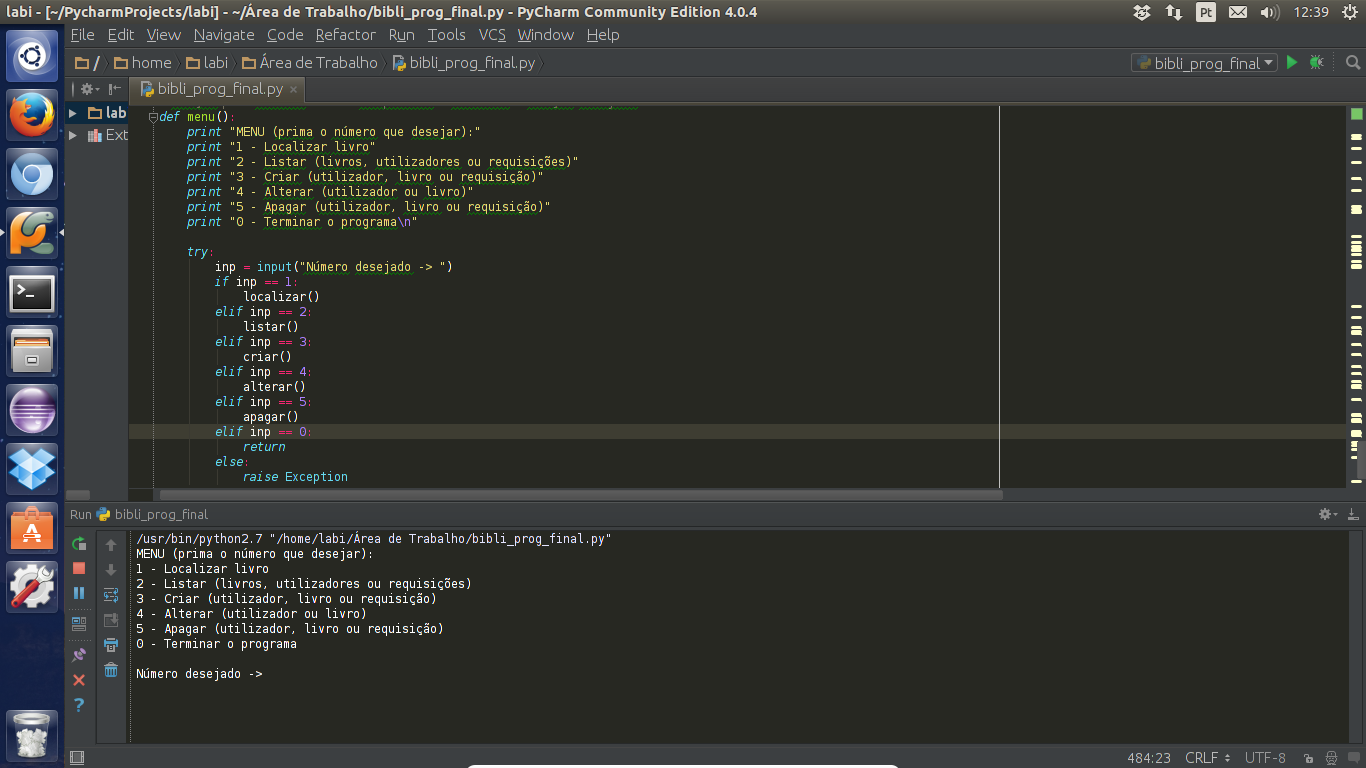
\includegraphics[scale=.35]{menu_principal.png}
 \caption{Menu principal funcional em baixo, com o seu código na metade superior da imagem}
 \label{menu_0}
\end{figure}

O programa inicia com um menu onde o utilizador é sugerido a inserir um número para escolher a operação que deseja realizar sobre a base de dados. Inicialmente, o utilizador tem cinco opções, para além da opção de terminar o programa (\autoref{menu_0}): 
\begin{enumerate}
\item Localizar um livro;
\item Listar livros, utilizadores ou requisições;
\item Criar utilizadores, livros ou requisições;
\item Alterar utilizadores ou livros;
\item Apagar utilizadores, livros ou requisições.
\end{enumerate}

\subsubsection{Menu "Localizar"}

A função localizar apresenta posteriormente um menu, para indicar se se pretende procurar por autor, título ou estado, e em último caso voltar ao menu inicial. Caso se queira pesquisar por autor ou por título, é preciso apenas uma parte da palavra a pesquisar para a encontrar, a uma ou a várias, com o padrão introduzido, devido à instrução "\%" antes e depois da palavra introduzida (\autoref{menu_1}). Caso seja escolhida a opção para pesquisar por estado, ainda apresenta mais um menu, que permite que se escolha entre listar os livros disponíveis e os requisitados.

\begin{figure}
 \center
 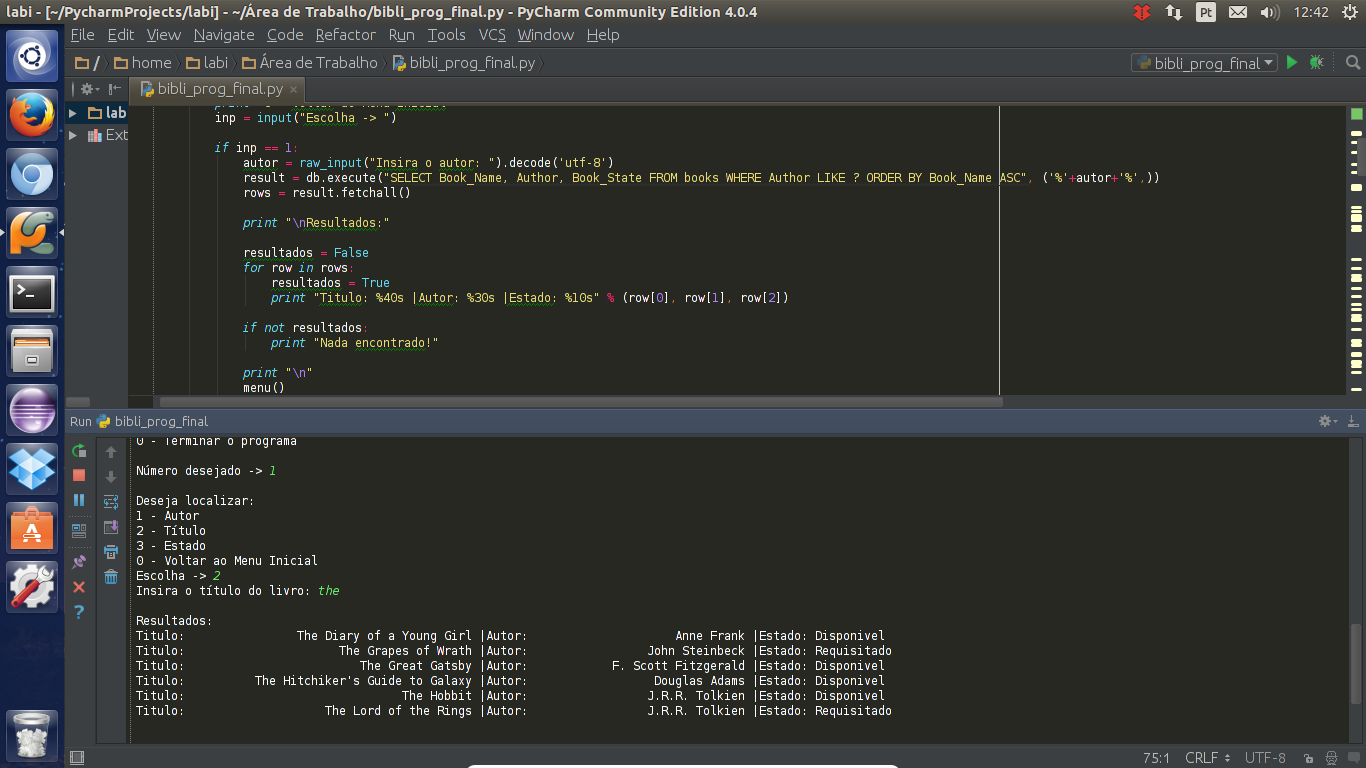
\includegraphics[scale=.35]{menu_1.png}
 \caption{Localizar livro, com o título contendo a palavra "the", com o seu código na metade superior da imagem}
 \label{menu_1}
\end{figure}

Quando a função acaba, tal como todas as outras funções criadas fora do menu, redireciona o utilizador de volta ao menu principal para optar por outras operações que deseja fazer.

\subsubsection{Menu "Listar"}

A função listar apresenta um menu com três opções disponíveis que permitem listar livros, utilizadores ou requisições, e em último caso voltar ao menu inicial. Caso o utilizador opte por listar livros (escolha "1"), o programa executa o comando para listar livros na base de dados e depois, um a um, lista-os com uma saída formatada, para ser mais simples ao utilizador ler a informação de cada livro. Caso escolhamos a opção de listar utilizadores (escolha "2"), executa o comando sobre a base de dados, lista todos os utilizadores, sendo eles todos imprimidos no visor.

No entanto, se a escolha do utilizador for listar requisições (escolha "3"), já não é assim tão simples como nas outras duas listagens. Neste caso, o utilizador terá primeiro de ler da base de dados todas as requisições existentes. Depois, guarda toda a informação (\textit{Id's} de livros, utilizadores e datas de requisição e limite) em listas, para depois ir procurar às respetivas tabelas (livros e utilizadores) o nome, título e autor correspondente. Finalmente, imprime todos estes dados (nome de utilizador, título de livro, autor, data de requisição e data limite de entrega) numa impressão formatada para o utilizador.

\subsubsection{Menu "Criar"}

No menu criar, é possível escolher entre listar utilizadores, livros e requisições, havendo também a possibilidade de voltar ao menu inicial. Se for pretendido criar utilizadores (escolha "1"), o programa irá pedir ao utilizador para introduzir um novo nome. É importante ser feita a descodificação para \textit{utf-8}, para ser possível ler utilizadores acentuados no nome. Depois, procura por utilizadores com esse nome. No caso de já existir, pede ao utilizador para escolher outro nome, pois não é possível haver dois nomes de utilizador iguais na base de dados criada. Caso não exista, insere-o na base de dados.
Se a escolha for criar livros (escolha "2"), o processo é semelhante. É pedido o título de um livro e o autor. O programa analisa a base de dados e se esse livro já existir, lança um erro. Caso não aconteça, insere o livro na base de dados, cujo o estado do livro em questão será "Disponível".

Se o utilizador optar por criar requisição (escolha "3"), o programa começa por pedir o nome de utilizador, o título do livro, o autor e a data limite de entrega de requisição. Se o utilizador não existir, se o livro não existir ou se já estiver requisitado, lança um erro. Caso contrário, adiciona à tabela de requisições o \textit{Id} do user, o \textit{Id} do livro (que são as chaves primárias das respetivas tabelas), a data atual e a data de limite de entrega inserida pelo utilizador. Por fim, altera também o estado do livro para "Requisitado".

\subsubsection{Menu "Alterar"}

A função alterar apresenta um sub-menu com três opções: alterar utilizador, alterar livro e voltar ao menu inicial. Caso queiramos alterar o utilizador, a aplicação começa por receber o nome que deseja ser alterado. Se esse nome não existe, lança um erro. Caso exista, recebe o novo nome, para o qual deseja ver alterado o utilizador. Depois, atualiza a base de dados com esse nome (\autoref{menu_2}).

\begin{figure}
 \center
 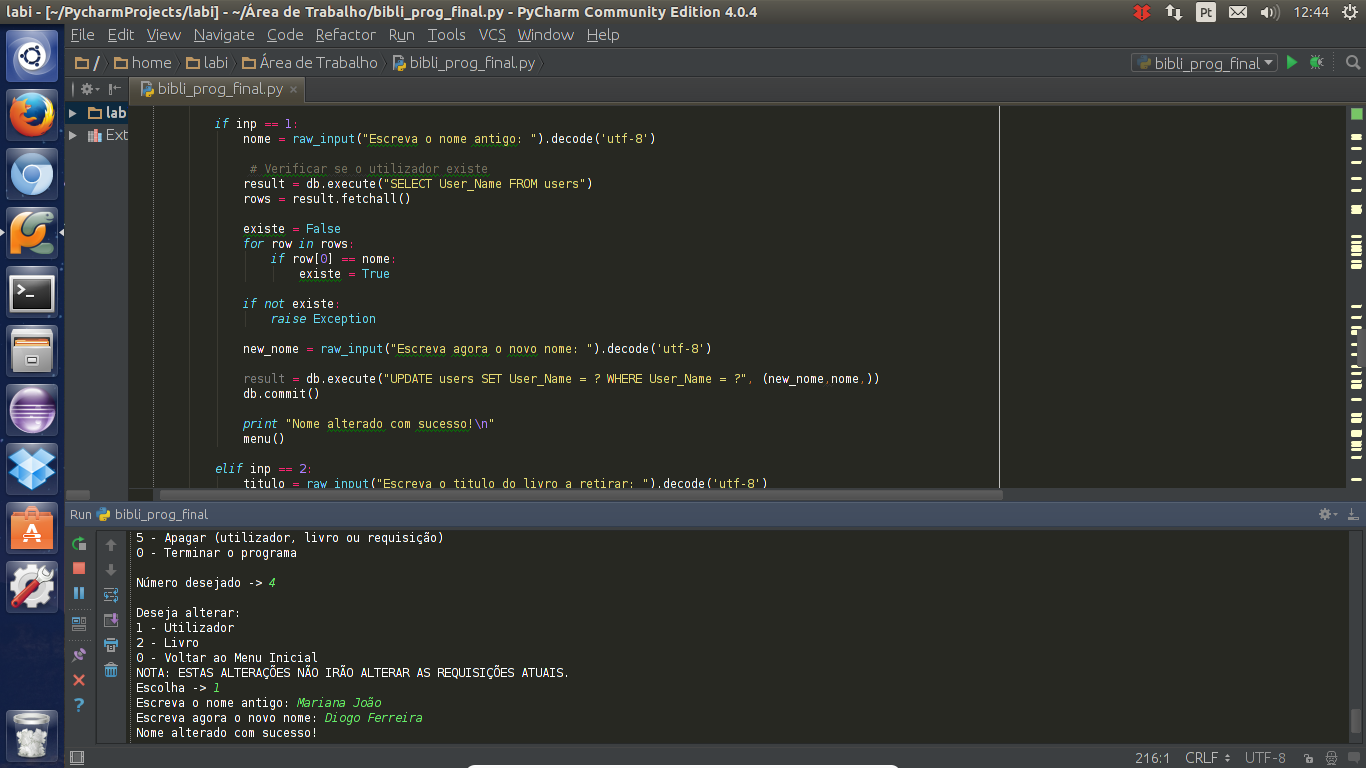
\includegraphics[scale=.35]{menu_2.png}
 \caption{Alterar nome de utilizador, de "Mariana João" para "Diogo Ferreira", com o seu código na metade superior da imagem}
 \label{menu_2}
\end{figure}


No caso do utilizador escolher alterar o livro (escolha "2"), começa por receber o título do livro e o seu autor e verificar se o livro existe na base de dados. Se não existir lança um erro. Caso contrário, recebe o novo título e o novo autor do livro, e atualiza a base de dados com esses dados.

\subsubsection{Menu "Apagar"}

Caso o utilizador pretenda apagar algum elemento da base de dados, ser-lhe-á exposto o sub-menu que apresenta as seguintes quatro opções: apagar utilizador, apagar livro, apagar requisição e voltar ao menu iniciar. Caso o utilizador escolha apagar um utilizador da base de dados, a aplicação começa por receber o nome do utilizador. Se ele não existir, lança erro. Caso contrário, procura na base de dados por possíveis requisições desse utilizador. Se existirem, apaga-as e altera o estado dos livros requisitados para disponível. Finalmente, após apagar todas as suas possíveis requisições, o utilizador é apagado da base de dados (\autoref{menu_3}).

\begin{figure}
 \center
 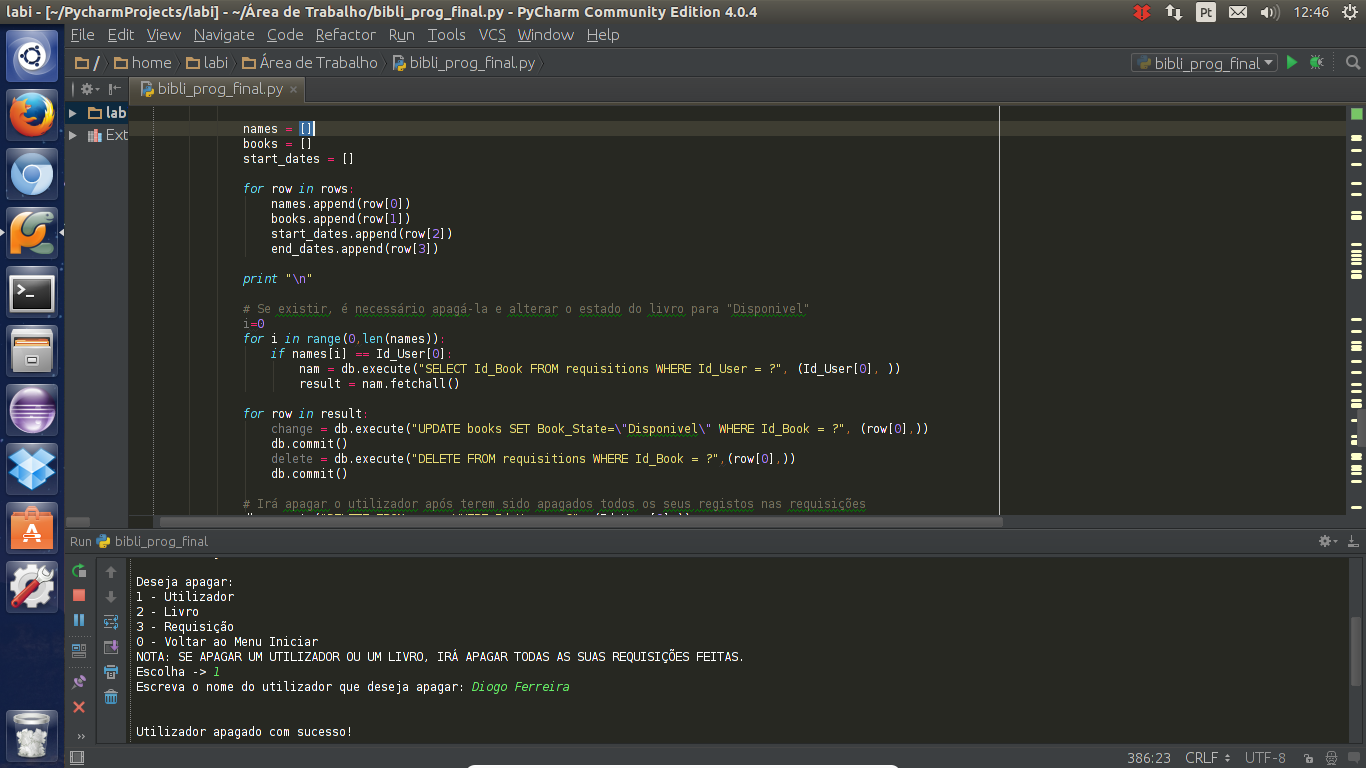
\includegraphics[scale=.35]{menu_3.png}
 \caption{Função de apagar utilizador, neste caso "Diogo Ferreira", com parte do seu código na metade superior da imagem}
 \label{menu_3}
\end{figure}

Se o utilizador escolher apagar o livro (escolha "2"), o programa começa por receber o título e o autor do livro que deseja apagar. Caso ele não exista, lança um erro. Caso exista, apaga todas as possíveis requisições com esse livro e depois apaga-o da base de dados.

Finalmente, se o utilizador escolher apagar uma requisição (escolha "3"), é pedido ao utilizador para introduzir o título e o autor do livro que deseja alterar o estado. Se o livro não existir, o programa lança um erro. Se existir, altera o seu estado para disponível e , caso exista, apaga as suas requisições.

\part{Conclusão}

\chapter{Conclusão}

As bases de dados são indispensáveis no mundo atual, onde informação é processada e exigida a todo o momento, sendo necessário uma forma de ser armazenada, protegida e de fácil acesso por parte dos utilizadores ou gestores. Elas permitem com que se possa estabelecer relações entre os mais variados dados introduzidos e manipulados. Conferem organização e consistência em formato digital. As aplicações ou conjuntos de programas que garantem que se desempenhem tarefas sobre as bases de dados são bastante importantes devido ao facto do tratamento de dados ser mais prático.

Com esta aplicação é pretendido fornecer um exemplo básico de uma ferramenta essencial para poder agir sobre uma base de dados de uma forma simplista e acessível a qualquer tipo de utilizador, sem quaisquer conhecimentos de programação ou outros conteúdos avançados. Reconhecemos que, apesar de tudo, é uma aplicação demasiado básica, a qual não consegue servir o utilizador em situações de maior detalhe e de manipulação de mais informação. No entanto, o nosso objetivo era o de expor uma aplicação não muito complicada, capaz de ser de fácil compreensão para qualquer utilizador, o que achamos que concluímos com sucesso.

\end{document}